\chapter{Исследовательская часть}
В текущем разделе будут представлены примеры работы разработанного программного обеспечения, постановка эксперимента и сравнительный анализ реализованных алгоритмов.

\section{Пример работы программного обеспечения}

На рисунках \ref{fig:prog_exmpl1}, \ref{fig:prog_exmpl2} представлен результат работы программы.

\begin{figure}[h!]
	
	\centering{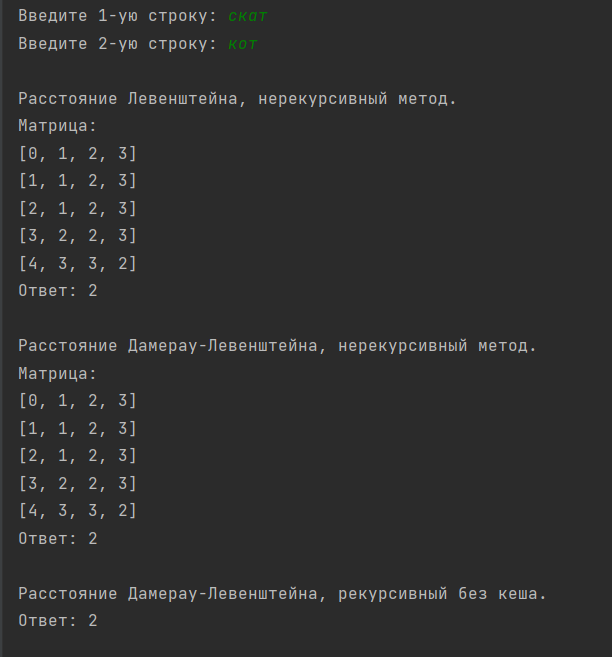
\includegraphics[scale=1]{inc/prog_exmpl1.PNG}}
	
	\caption{Пример работы программы}
	
	\label{fig:prog_exmpl1}
	
\end{figure}

\begin{figure}[h!]
	
	\centering{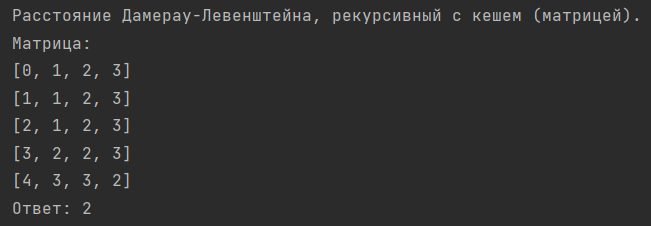
\includegraphics[scale=1]{inc/prog_exmpl2.PNG}}
	
	\caption{Пример работы программы}
	
	\label{fig:prog_exmpl2}
	
\end{figure}

\section{Технические характеристики}

Технические характеристики устройства, на котором выполнялось тестирование:

\begin{itemize}
	\item операционная система: Windows 10~\cite{windows10};
	\item оперативная память: 16 Гб;
	\item процессор: Intel® Core™ i5 10300H 2.5 ГГц.
\end{itemize}

Во время тестирования ноутбук был включен в сеть питания и нагружен только встроенными приложениями окружения и системой тестирования.

\section{Время выполнения реализаций алгоритмов}

Замеры процессорного времени реализованных алгоритмов поиска расстояний Левенштейна и Дамерау-Левенштейна проводились с помощью функции process\_time() из библиотеки time языка Python. 

Функция process\_time() возвращает время в секундах (сумму системного и пользовательского процессорного времени).

Замеры времени для каждой длины слов (от 0 до 9 символов) проводились 1e5 раз для нерекурсивных алгоритмов поиска расстояния Левенштейна и Дамерау-Левенштейна, 100 раз для рекурсивных (с кешированием и без) алгоритмов поиска расстояния Дамерау-Левенштейна. В качестве результата бралось среднее время работы алгоритма на каждой длине слова.

На рисунке \ref{fig:fig1} представлен график сравнения реализаций нерекурсивных алгоритмов поиска расстояний Левенштейна и Дамерау-Левенштейна. На графике видно, что оба алгоритма практически одинаково эффективны по времени, но чуть менее эффективен алгоритм поиска расстояния Дамерау-Левенштейна (с длины слова равной 4) из-за дополнительной операции обмена двух соседних символов.


На рисунке \ref{fig:fig2} представлен график сравнения реализаций рекурсивных алгоритмов (с кешированием и без) поиска расстояния Дамерау-Левенштейна. На графике видно, что полученные результаты почти накладываются друг на друга до длины слова равной 6, но при большей длине слова рекурсивный алгоритм Дамерау-Левенштейна с кешированием значительно эффективнее по времени, так как за счет кеша в виде матрицы не производится повторных вычислений (отсутствие вызова функций для вычисления значений, которые уже были посчитаны ранее).


На рисунке \ref{fig:fig3} представлен график сравнения всех реализованных в рамках лабораторной работы алгоритмов поиска расстония Левенштейна и Дамерау-Левенштейна. На графике видно, что при длине слова больше 6 символов самым неэффективным алгоритмом является рекурсивный алгоритм поиска расстояния Дамерау-Левенштейна без кеширования из-за большого количества повторных вычислений.

\section{Оценка затрат алгоритмов по памяти}

Алгоритмы поиска расстояний Левенштейна и Дамерау-Левенштейна затрачивают схожее количество памяти, но оно будет варьироваться при использовании разных подходов (итеративный, рекурсивный).

Пусть длина строки $S_1$ - m, длина строки $S_2$ - n, тогда затраты памяти на приведенные выше алгоритмы будут следующими.

Итерационный алгоритмы поиска расстояния Левенштейна и Дамерау-Левенштейна:\\
\begin{itemize}
\item матрица - ((m + 1) * (n + 1)) * sizeof(int); 
\item строки $S_1$, $S_2$ - (m + n) * sizeof(char); 
\item длины строк - 2 * sizeof(int); 
\item вспомогательные переменные -  3 * sizeof(int); (для Дамерау-Левенштейна - 4 * sizeof(int))
\end{itemize}

Максимальная глубина стека вызовов при рекурсивной реализации равна сумме длин входящих строк.

Затраты по памяти для каждого рекурсивного вызова:
\begin{itemize}
	\item рекурсивный алгоритм поиска расстояния Дамерау-Левенштейна без кеширования:\begin{itemize}
		\item строки $S_1$, $S_2$ - (m + n) * sizeof(char);
		\item длины строк $S_1$, $S_2$ - 2 * sizeof(int);
		\item вспомогательные переменные -  4 * sizeof(int);
		\item адрес возврата;
	\end{itemize}
	\item рекурсивный алгоритм поиска расстояния Дамерау-Левенштейна с кешированием: \begin{itemize}
	    \item матрица - ((m + 1) * (n + 1)) * sizeof(int); (1 раз)
		\item строки $S_1$, $S_2$ - (m + n) * sizeof(char);
		\item длины строк $S_1$, $S_2$ - 2 * sizeof(int);
		\item вспомогательная переменная -  1 * sizeof(int);
		\item указатель на матрицу - 1 * sizeof(int*);
		\item адрес возврата;
	\end{itemize}
\end{itemize}

\section*{Вывод}

Реализации итерационных алгоритмов поиска расстояний Левенштейна и Дамерау — Левенштейна почти одинаково эффективны по времени, но при увеличении длины слова незначительно больше времени затрачивает алгоритм поиска расстояния Дамерау-Левенштейна из-за дополнительной операции обмена двух соседних символов, но она довольно часто позволяет найти более короткое расстояние между строками.

Рекурсивный алгоритм нахождения расстояния Дамерау-Левенштейна без кеширования работает намного дольше рекурсивного алгоритма с кешированием и итеративного алгоритма поиска расстояния Дамерау-Левенштейна. Рекурсивный алгоритм с кешированием требует меньше времени, однако требует больше времени, чем итерационный алгоритм поиска расстояния Дамерау-Левенштейна, причем чем больше длина строки, тем больше разрыв по времени. 

По количеству затрачиваемой памяти итеративные алгоритмы проигрывают рекурсивным без кеширования (максимальный размер используемой памяти в итеративных алгоритмах пропорционален произведению длин строк, в рекурсивныхбез кеширования — сумме длин строк).

\begin{figure}[h!]
	
	\centering{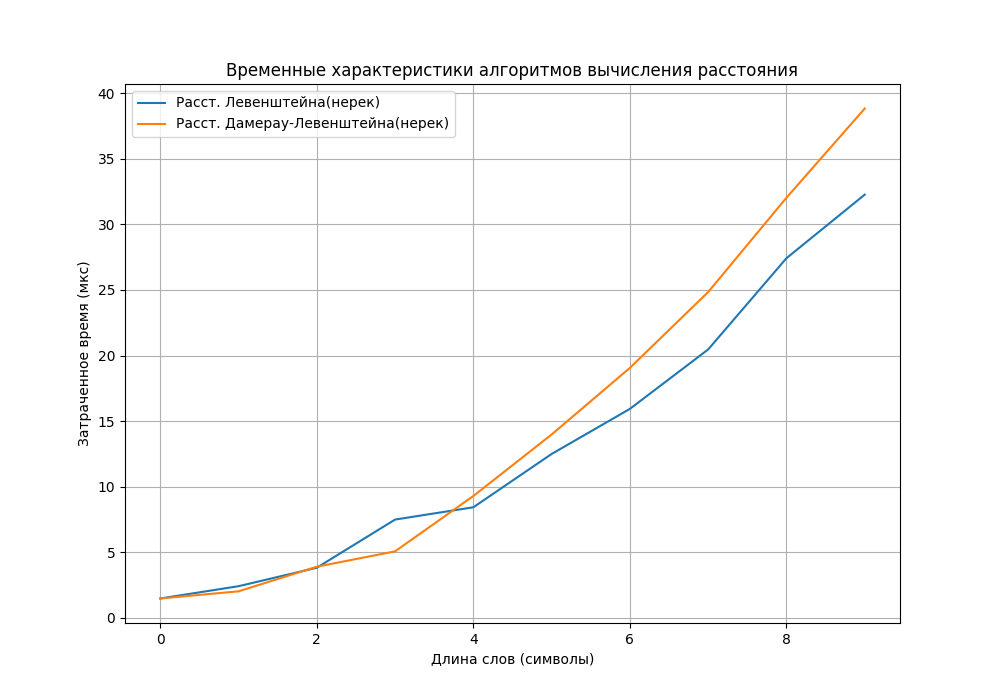
\includegraphics[scale=0.6]{inc/Figure_1.png}}
	
	\caption{График сравнения реализаций нерекурсивных алгоритмов поиска расстояний Левенштейна и Дамерау-Левенштейна}
	
	\label{fig:fig1}
	
\end{figure}
	
\begin{figure}[h!]
	
	\centering{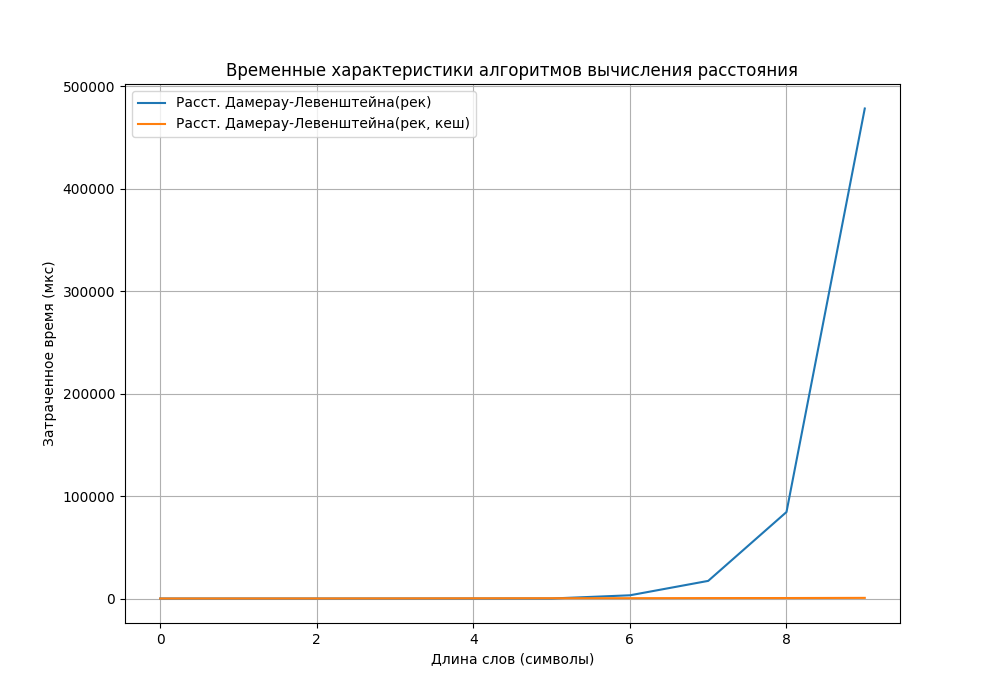
\includegraphics[scale=0.6]{inc/Figure_2.png}}
	
	\caption{График сравнения реализаций рекурсивных алгоритмов (с кешированием и без) поиска расстояния Дамерау-Левенштейна}
	
	\label{fig:fig2}
	
\end{figure}


\begin{figure}[h!]
	
	\centering{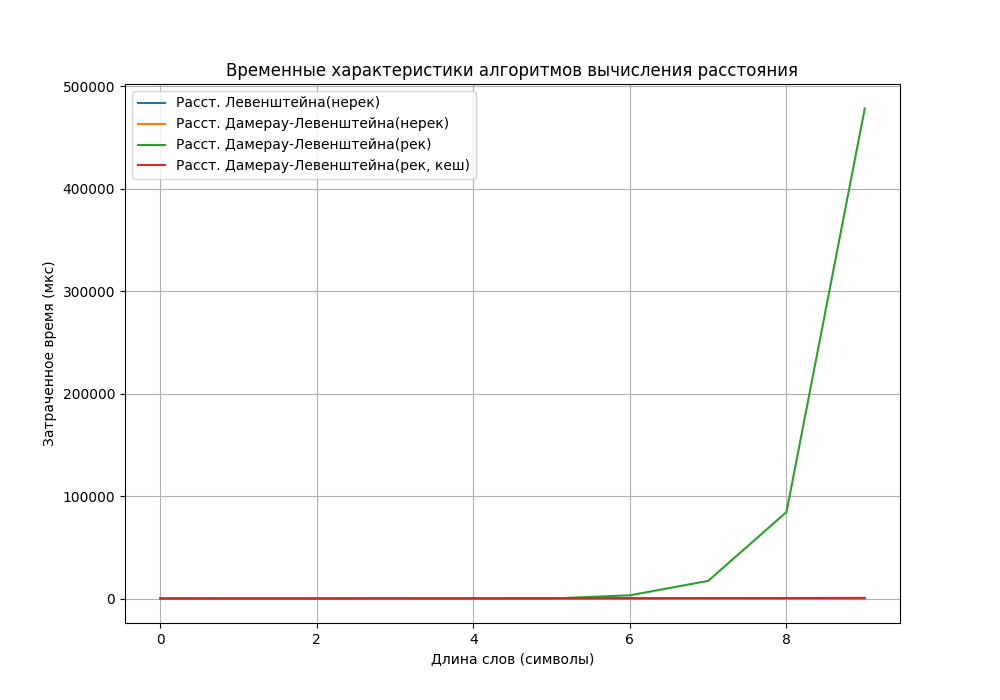
\includegraphics[scale=0.6]{inc/Figure_3.png}}
	
	\caption{График сравнения алгоритмов поиска расстоний Левенштейна и Дамерау-Левенштейна}
	
	\label{fig:fig3}
	
\end{figure}